\documentclass[8pt,twocolumn,a4paper]{extarticle}

% =========================================================
% YELLOW.AI - TECHQUEST
% NEXUS LOOP
% ENDTERM / FINAL TECHNICAL REPORT TEMPLATE
% =========================================================

% ---------------------------------------------------------
% PACKAGES
% ---------------------------------------------------------

\usepackage[english]{babel}
\usepackage[utf8]{inputenc}
\usepackage[T1]{fontenc}

% Page size and margins
\usepackage[
    a4paper,
    top=1.35cm,
    bottom=1.35cm,
    left=1.45cm,
    right=1.45cm
]{geometry}

% Mathematics
\usepackage{amsmath}
\usepackage{amssymb}

% Tables and figures
\usepackage{graphicx}
\usepackage{booktabs}
\usepackage{array}
\usepackage{multirow}
\usepackage{caption}

% Lists
\usepackage{enumitem}

% Links
\usepackage[colorlinks=true,allcolors=blue]{hyperref}

% Better spacing
\usepackage{microtype}

% ---------------------------------------------------------
% COMPACT FORMATTING
% ---------------------------------------------------------

\setlength{\parindent}{0pt}
\setlength{\parskip}{2pt}

\setlist[itemize]{
    leftmargin=*,
    nosep,
    topsep=1pt,
    partopsep=0pt
}

\setlist[enumerate]{
    leftmargin=*,
    nosep,
    topsep=1pt,
    partopsep=0pt
}

\captionsetup{
    font=small,
    labelfont=bf,
    skip=3pt
}

% ---------------------------------------------------------
% TITLE
% ---------------------------------------------------------

\title{
    \normalfont
    \normalsize
    \textsc{TECHQUEST} \\[3pt]
    \Large \textbf{Nexus Loop} \\[2pt]
    \normalsize
    \textit{Building an Autonomous Improvement Loop for AI Agent Deployments}
}

\author{
    \textbf{Team Name:} [TEAM NAME]
    \\
    \textbf{Team ID:} [TEAM ID]
    \\
    \textbf{Institution:} [INSTITUTION]
}

\date{}

% =========================================================
% DOCUMENT
% =========================================================

\begin{document}

\maketitle

% =========================================================
% ABSTRACT
% =========================================================

\begin{abstract}

We present \textbf{[SYSTEM NAME]}, an autonomous improvement loop for
AI-agent deployments that converts execution logs into actionable
diagnoses and verified improvement proposals. The system follows the
\textbf{Detect $\rightarrow$ Diagnose $\rightarrow$ Prescribe
$\rightarrow$ Verify} workflow. It identifies genuine regressions,
dismisses lookalike changes, quantifies their impact with explicit
fidelity and coverage, identifies likely causes and responsible
configuration changes, proposes fixes, evaluates them using the replay
service, and records the final human decision. On the sealed dataset,
the system achieves \textbf{[KEY RESULT]} with \textbf{[RUNTIME]} runtime
and \textbf{[COVERAGE]} coverage. We additionally report measurement
gaps, judge calibration, failure cases, and the limitations of the
system at larger scale.

\end{abstract}

\noindent
\textbf{Keywords:}
Agent Observability, Root Cause Analysis, AI Agents, Autonomous
Improvement, Anomaly Detection, Evaluation, Human-in-the-Loop

% =========================================================
% 1. PROBLEM AND OBJECTIVE
% =========================================================

\section{Problem and Objective}

AI-agent deployments generate large volumes of execution data including
conversations, tool calls, model information, outcomes, transcripts,
and configuration changes. The challenge is to turn these logs into a
closed improvement loop rather than relying on manual investigation.

Our system addresses four stages:

\begin{enumerate}
    \item \textbf{Detect:} identify genuine problems and affected
    traffic slices.
    \item \textbf{Diagnose:} determine why the problem occurred and
    identify the relevant configuration change.
    \item \textbf{Prescribe:} propose a concrete fix and state its
    associated risk.
    \item \textbf{Verify:} replay the affected cohort and determine
    whether the fix actually improves the outcome.
\end{enumerate}

The system is designed to answer the operator's core questions:
\textit{What broke? Who was affected? Why did it happen? Who should
act? What happens if nobody acts? Can the proposed fix be trusted?}

% ---------------------------------------------------------
% 1.1 Objectives
% ---------------------------------------------------------

\subsection{Objectives}

The primary objectives of the system are:

\begin{itemize}
    \item Detect genuine regressions from deployment logs.
    \item Identify the precise traffic slice affected.
    \item Quantify impact using defensible denominators.
    \item Diagnose the underlying cause.
    \item Link diagnoses to relevant configuration changes.
    \item Explicitly dismiss lookalike / false-alarm patterns.
    \item Refuse questions that cannot be answered from available data.
    \item Mine the deployment's own ``good'' behaviour as a standard.
    \item Propose and verify fixes through replay.
    \item Keep a human approval/rejection decision in the loop.
\end{itemize}

% =========================================================
% 2. DATA AND SYSTEM UNDERSTANDING
% =========================================================

\section{Data and System Understanding}

\subsection{Available Data}

The system operates on the provided deployment corpus containing:

\begin{itemize}
    \item 80,000 conversations;
    \item 880,000 execution steps;
    \item Conversation transcripts;
    \item 16 timestamped configuration changes;
    \item Sparse human ratings;
    \item Human resolution labels and quality scores.
\end{itemize}

The system initially uses the provided sample dataset for development
and subsequently confirms reported findings on the full corpus.

\subsection{Data Model and Joins}

Describe the relevant entities, fields, relationships, and safe joins
used by the system.

\begin{table}[h]
\centering
\caption{Important data entities and their usage.}
\label{tab:data}
\small
\begin{tabular}{p{0.28\columnwidth}p{0.62\columnwidth}}
\toprule
\textbf{Entity} & \textbf{Usage} \\
\midrule
Conversation & [Purpose / fields used] \\
Execution step & [Purpose / fields used] \\
Transcript & [Purpose / fields used] \\
Configuration & [Purpose / fields used] \\
Human labels & [Purpose / fields used] \\
Ratings & [Purpose / fields used] \\
\bottomrule
\end{tabular}
\end{table}

\subsection{Measurement Constraints}

State explicitly which quantities can and cannot be measured from the
available logs.

For every reported metric, distinguish:

\begin{itemize}
    \item \textbf{Fidelity:} measured, derived, or judged;
    \item \textbf{Coverage:} fraction of traffic for which the metric
    can actually be computed;
    \item \textbf{Calibration:} agreement with human labels for judged
    quantities.
\end{itemize}

% =========================================================
% 3. SYSTEM OVERVIEW
% =========================================================

\section{System Overview}

\subsection{Architecture}

Describe the complete automated pipeline from raw deployment logs to
the final report and decision layer.

\begin{figure}[t]
    \centering
    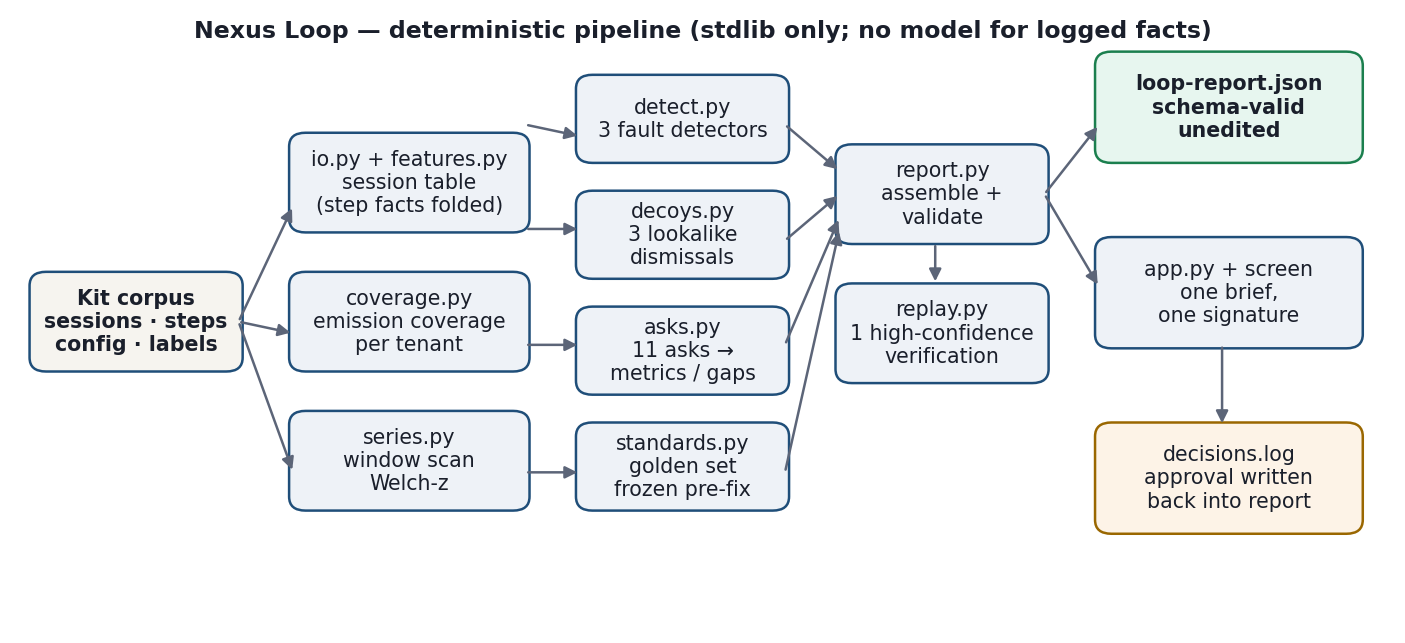
\includegraphics[width=0.98\columnwidth]
    {figures/system_architecture.png}
    \caption{
        Overall architecture of the proposed Nexus Loop system.
    }
    \label{fig:architecture}
\end{figure}

\subsection{End-to-End Pipeline}

The implemented pipeline consists of:

\begin{enumerate}
    \item \textbf{Data ingestion and validation}
    \item \textbf{Metric computation}
    \item \textbf{Traffic slicing}
    \item \textbf{Problem detection}
    \item \textbf{False-alarm analysis}
    \item \textbf{Root-cause diagnosis}
    \item \textbf{Impact estimation}
    \item \textbf{Standard mining}
    \item \textbf{Fix prescription}
    \item \textbf{Replay verification}
    \item \textbf{Human decision}
    \item \textbf{Report generation}
\end{enumerate}

Replace the above with the actual implementation if the ordering or
components differ.

% =========================================================
% 4. DETECTION
% =========================================================

\section{Detection}

\subsection{Metrics}

Describe the metrics used to detect changes in agent behaviour.

\begin{table}[h]
\centering
\caption{Primary metrics used by the detection system.}
\label{tab:metrics}
\small
\begin{tabular}{p{0.24\columnwidth}p{0.27\columnwidth}p{0.35\columnwidth}}
\toprule
\textbf{Metric} & \textbf{Definition} & \textbf{Fidelity / Coverage} \\
\midrule
[Metric 1] & [Definition] & [Measured / Derived / Judged] \\
[Metric 2] & [Definition] & [Measured / Derived / Judged] \\
[Metric 3] & [Definition] & [Measured / Derived / Judged] \\
\bottomrule
\end{tabular}
\end{table}

\subsection{Detection Strategy}

Explain:

\begin{itemize}
    \item How traffic is grouped into meaningful cohorts;
    \item How baselines are selected;
    \item How temporal changes are detected;
    \item How thresholds are selected;
    \item How insufficient sample sizes are handled;
    \item How the system distinguishes signal from normal variation.
\end{itemize}

\subsection{Affected Slice}

For each detected problem, report the exact slice in which the
behaviour occurs.

Examples of useful dimensions include:

\begin{itemize}
    \item Intent;
    \item Tenant;
    \item Time period;
    \item Model / agent version;
    \item Tool usage;
    \item Other relevant traffic attributes.
\end{itemize}

% =========================================================
% 5. FINDINGS AND SPECIFICITY
% =========================================================

\section{Findings}

\subsection{Real Problems}

For every genuine problem, provide an explicit impact block.

\begin{table}[h]
\centering
\caption{Summary of genuine findings.}
\label{tab:findings}
\small
\begin{tabular}{p{0.15\columnwidth}p{0.23\columnwidth}p{0.48\columnwidth}}
\toprule
\textbf{ID} & \textbf{Affected Slice} & \textbf{Finding / Impact} \\
\midrule
F-01 & [Slice] & [What changed and who was affected] \\
F-02 & [Slice] & [What changed and who was affected] \\
F-03 & [Slice] & [What changed and who was affected] \\
\bottomrule
\end{tabular}
\end{table}

For each finding, state:

\begin{itemize}
    \item Number of affected conversations;
    \item Percentage of total traffic;
    \item Change in the relevant outcome;
    \item Number of users negatively affected;
    \item Additional human handoffs, if applicable;
    \item Duration of the problem;
    \item Estimated consequence / cost;
    \item Responsible owner;
    \item Consequence of taking no action.
\end{itemize}

\subsection{False Alarms / Lookalikes}

The system must explicitly explain why observed changes were \textbf{not}
classified as regressions.

\begin{table}[h]
\centering
\caption{Lookalikes examined and rejected.}
\label{tab:lookalikes}
\small
\begin{tabular}{p{0.18\columnwidth}p{0.31\columnwidth}p{0.41\columnwidth}}
\toprule
\textbf{Case} & \textbf{Observed Change} & \textbf{Reason Dismissed} \\
\midrule
L-01 & [Pattern] & [Evidence] \\
L-02 & [Pattern] & [Evidence] \\
L-03 & [Pattern] & [Evidence] \\
\bottomrule
\end{tabular}
\end{table}

Explain the evidence that distinguishes each lookalike from a genuine
regression.

% =========================================================
% 6. DIAGNOSIS
% =========================================================

\section{Diagnosis}

\subsection{Root-Cause Analysis}

For each real problem, explain the causal reasoning used to move from
the observed symptom to the underlying cause.

\begin{figure}[h]
    \centering
    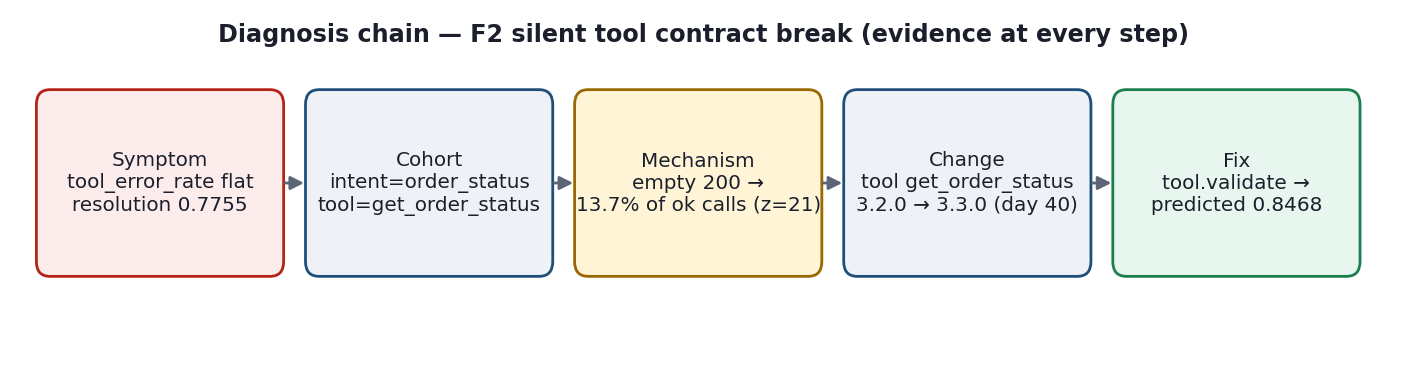
\includegraphics[width=0.98\columnwidth]
    {figures/diagnosis.png}
    \caption{
        Example diagnosis chain from observed regression to responsible
        configuration change.
    }
    \label{fig:diagnosis}
\end{figure}

The diagnosis should identify:

\begin{enumerate}
    \item Observed metric change;
    \item Affected cohort;
    \item Relevant temporal window;
    \item Candidate causes;
    \item Evidence supporting the selected cause;
    \item Configuration change responsible, where applicable.
\end{enumerate}

\subsection{Baseline Selection}

Clearly state the baseline used for each diagnosis.

Where a before-period exists, explain the before/after comparison.

Where no before-period exists, explain the peer or deployment-internal
baseline used instead.

\subsection{Configuration Change Attribution}

For every attributed configuration change, report:

\begin{itemize}
    \item Configuration identifier;
    \item Timestamp;
    \item Parameter / component changed;
    \item Previous state;
    \item New state;
    \item Relationship to the detected regression;
    \item Evidence supporting the attribution.
\end{itemize}

% =========================================================
% 7. MEASUREMENT GAPS
% =========================================================

\section{Measurement Gaps}

This section documents questions that the available data cannot answer.

\subsection{Unanswerable Questions}

For every refused question, explicitly state:

\begin{enumerate}
    \item The question;
    \item Why the available logs cannot answer it;
    \item Which event or field is missing;
    \item The exact event that would need to be logged;
    \item How that event would enable future measurement.
\end{enumerate}

\begin{table}[h]
\centering
\caption{Measurement gaps.}
\label{tab:gaps}
\small
\begin{tabular}{p{0.24\columnwidth}p{0.34\columnwidth}p{0.32\columnwidth}}
\toprule
\textbf{Question} & \textbf{Why Unanswerable} & \textbf{Required Event} \\
\midrule
[Axx] & [Reason] & [Required event] \\
[Question] & [Reason] & [Required event] \\
\bottomrule
\end{tabular}
\end{table}

Do not infer or estimate quantities for which the required event is not
present in the data.

% =========================================================
% 8. STANDARD / GOOD BEHAVIOUR
% =========================================================

\section{Deployment Standard}

\subsection{Mining ``Good'' Behaviour}

Describe how the system identifies high-quality conversations from the
deployment itself and converts them into a reference standard.

The standard should capture:

\begin{itemize}
    \item Relevant behavioural characteristics;
    \item Expected resolution behaviour;
    \item Expected conversation length;
    \item Tool usage patterns;
    \item Quality indicators;
    \item Other deployment-specific properties.
\end{itemize}

\subsection{Deviation from Standard}

Explain how observed problematic cohorts are compared against the
deployment's own good behaviour.

\begin{figure}[h]
    \centering
    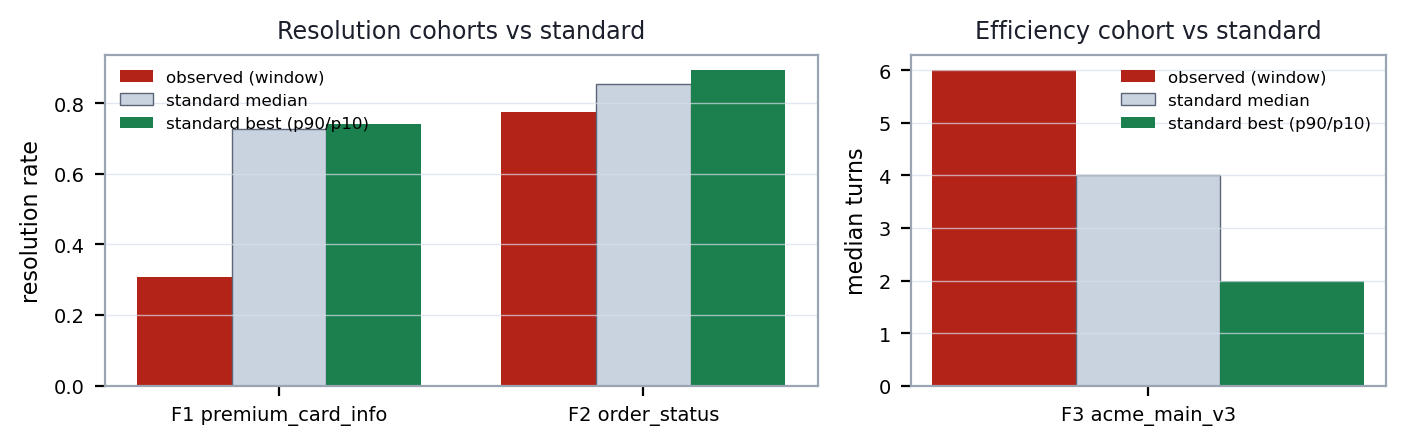
\includegraphics[width=0.98\columnwidth]
    {figures/standard_comparison.png}
    \caption{
        Comparison between the mined deployment standard and an affected
        cohort.
    }
    \label{fig:standard}
\end{figure}

% =========================================================
% 9. PRESCRIPTION
% =========================================================

\section{Prescription}

\subsection{Proposed Fix}

For each real problem, describe one concrete proposed intervention.

\begin{table}[h]
\centering
\caption{Proposed fixes.}
\label{tab:fixes}
\small
\begin{tabular}{p{0.13\columnwidth}p{0.28\columnwidth}p{0.43\columnwidth}}
\toprule
\textbf{ID} & \textbf{Problem} & \textbf{Proposed Fix} \\
\midrule
P-01 & [Finding ID] & [Fix description] \\
P-02 & [Finding ID] & [Fix description] \\
\bottomrule
\end{tabular}
\end{table}

\subsection{Risk and Shipping Criteria}

Every proposed fix must state:

\begin{itemize}
    \item What change is being proposed;
    \item Why it should address the diagnosed cause;
    \item Risk if the diagnosis is wrong;
    \item What metric(s) should improve;
    \item What would prevent the fix from being shipped;
    \item Conditions under which the fix should be rejected.
\end{itemize}

The system proposes changes to the agent, but never changes the
evaluation yardstick.

% =========================================================
% 10. VERIFICATION
% =========================================================

\section{Verification}

\subsection{Replay Method}

Describe how the proposed fix is submitted to the replay service and
how the affected cohort is selected.

The verification must compare:

\begin{itemize}
    \item Before-fix behaviour;
    \item After-fix behaviour;
    \item Relevant outcome metrics;
    \item Statistical / practical significance where applicable;
    \item Any regressions introduced by the fix.
\end{itemize}

\subsection{Before--After Results}

\begin{table}[h]
\centering
\caption{Replay verification results.}
\label{tab:replay}
\small
\begin{tabular}{p{0.20\columnwidth}ccc}
\toprule
\textbf{Metric} & \textbf{Before} & \textbf{After} & \textbf{Change} \\
\midrule
[Metric 1] & [X] & [X] & [X] \\
[Metric 2] & [X] & [X] & [X] \\
[Metric 3] & [X] & [X] & [X] \\
\bottomrule
\end{tabular}
\end{table}

A fix returning no measurable effect must be reported as a valid
negative result rather than being hidden.

\subsection{Verification Decision}

State whether the proposed fix:

\begin{itemize}
    \item \textbf{Worked and should be considered for deployment;}
    \item \textbf{Did not produce the expected effect;}
    \item \textbf{Introduced unacceptable side effects;}
    \item \textbf{Requires additional testing.}
\end{itemize}

% =========================================================
% 11. HUMAN DECISION LAYER
% =========================================================

\section{Decision Layer}

\subsection{Approve / Reject Workflow}

Describe how a human operator reviews:

\begin{enumerate}
    \item The finding;
    \item Evidence and impact;
    \item Diagnosis;
    \item Proposed fix;
    \item Verification result;
    \item Associated risk.
\end{enumerate}

The final screen must provide a working:

\begin{center}
\textbf{APPROVE \qquad / \qquad REJECT}
\end{center}

control and write the human decision back into the report.

\subsection{Decision Record}

\begin{table}[h]
\centering
\caption{Human decisions for proposed fixes.}
\label{tab:decisions}
\small
\begin{tabular}{p{0.16\columnwidth}p{0.20\columnwidth}p{0.45\columnwidth}}
\toprule
\textbf{Fix} & \textbf{Decision} & \textbf{Reason} \\
\midrule
P-01 & [Approve/Reject] & [Human reasoning] \\
P-02 & [Approve/Reject] & [Human reasoning] \\
\bottomrule
\end{tabular}
\end{table}

A rejection supported by a strong reason should be treated as a valid
decision, not a failed outcome.

% =========================================================
% 12. SELF-ASSESSMENT
% =========================================================

\section{Self-Assessment}

Describe how the system evaluates its own performance.

\subsection{Detection Performance}

Report:

\begin{itemize}
    \item Genuine problems detected;
    \item Genuine problems missed;
    \item False alarms;
    \item Detection hit rate;
    \item Detection latency.
\end{itemize}

\subsection{Judge Calibration}

If a model is used for semantic judgement, report:

\begin{itemize}
    \item Judge model / version;
    \item Judgement task;
    \item Human-labelled evaluation set;
    \item Agreement with human labels;
    \item Calibration methodology.
\end{itemize}

Do not report a calibration of 1.00 without explaining the evaluation
procedure and dataset.

\subsection{End-to-End Loop Completeness}

Report which stages execute automatically:

\begin{table}[h]
\centering
\caption{Automation coverage of the improvement loop.}
\label{tab:loop}
\small
\begin{tabular}{p{0.25\columnwidth}p{0.19\columnwidth}p{0.43\columnwidth}}
\toprule
\textbf{Stage} & \textbf{Automated?} & \textbf{Implementation} \\
\midrule
Detect & [Yes/No] & [Description] \\
Diagnose & [Yes/No] & [Description] \\
Prescribe & [Yes/No] & [Description] \\
Verify & [Yes/No] & [Description] \\
Decision & Human & [Interface / storage] \\
\bottomrule
\end{tabular}
\end{table}

% =========================================================
% 13. IMPLEMENTATION
% =========================================================

\section{Implementation}

\subsection{Technology Stack}

\begin{table}[h]
\centering
\caption{Implementation stack.}
\label{tab:stack}
\small
\begin{tabular}{p{0.29\columnwidth}p{0.57\columnwidth}}
\toprule
\textbf{Component} & \textbf{Implementation} \\
\midrule
Language & [Python / etc.] \\
Data processing & [Libraries / implementation] \\
Detection & [Method] \\
Diagnosis & [Method] \\
Semantic judgement & [Model / version] \\
Replay & [Implementation] \\
Screen & [Framework] \\
Report generation & [Implementation] \\
Storage & [Implementation] \\
\bottomrule
\end{tabular}
\end{table}

\subsection{Report Generation}

The final \texttt{loop-report.json} is generated directly by the system
and validated against the provided schema.

Describe:

\begin{itemize}
    \item Report generation;
    \item Schema validation;
    \item Evidence storage;
    \item Human decision persistence;
    \item Error handling.
\end{itemize}

\subsection{Execution Environment}

State the exact environment required to execute the system:

\begin{itemize}
    \item Operating environment;
    \item Python version;
    \item Dependencies;
    \item Docker image;
    \item CPU / memory requirements;
    \item Offline execution requirements.
\end{itemize}

% =========================================================
% 14. COMPUTATIONAL EFFICIENCY
% =========================================================

\section{Computational Efficiency}

\subsection{Runtime and Memory}

\begin{table}[h]
\centering
\caption{Computational performance.}
\label{tab:compute}
\small
\begin{tabular}{p{0.50\columnwidth}c}
\toprule
\textbf{Metric} & \textbf{Value} \\
\midrule
Average runtime / sealed scenario & [X] sec \\
Best runtime & [X] sec \\
Worst runtime & [X] sec \\
Peak memory & [X] MB \\
Dataset preprocessing time & [X] sec \\
Map / index / cache size & [X] MB \\
\bottomrule
\end{tabular}
\end{table}

\subsection{Bottlenecks}

Identify the dominant computational bottlenecks and explain the
optimizations used.

Examples include:

\begin{itemize}
    \item Precomputation;
    \item Indexing;
    \item Cohort pruning;
    \item Caching;
    \item Vectorization;
    \item Parallel processing;
    \item Coarse-to-fine analysis.
\end{itemize}

% =========================================================
% 15. RESULTS
% =========================================================

\section{Final Results}

\subsection{Overall Performance}

Summarize the final system performance on the sealed run.

\begin{table}[h]
\centering
\caption{Final system performance.}
\label{tab:results}
\small
\begin{tabular}{p{0.46\columnwidth}c}
\toprule
\textbf{Metric} & \textbf{Result} \\
\midrule
Diagnostic accuracy & [X] \\
False alarms & [X] \\
Metric coverage & [X]\% \\
Detection hit rate & [X]\% \\
Loop completeness & [X]\% \\
Average runtime / scenario & [X] sec \\
Peak memory & [X] MB \\
\bottomrule
\end{tabular}
\end{table}

\subsection{Evidence Summary}

Include the most important evidence supporting the final result.

\begin{figure}[h]
    \centering
    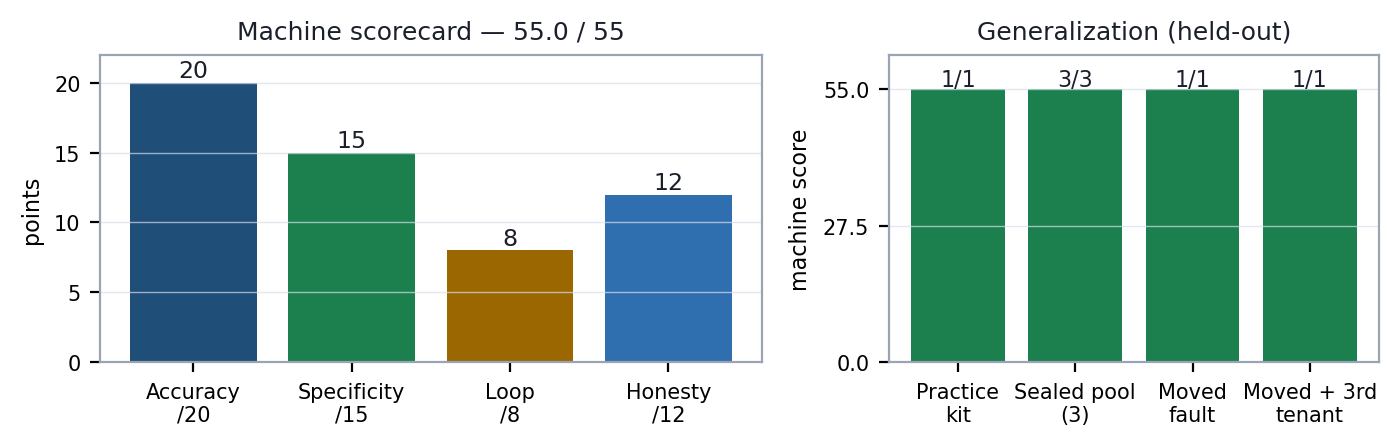
\includegraphics[width=0.98\columnwidth]
    {figures/results.png}
    \caption{
        Summary of final detection, diagnosis, and verification results.
    }
    \label{fig:results}
\end{figure}

% =========================================================
% 16. SCREEN / OPERATOR EXPERIENCE
% =========================================================

\section{Operator Screen}

The system provides one actionable screen rather than a collection of
engineering dashboards.

\begin{figure}[h]
    \centering
    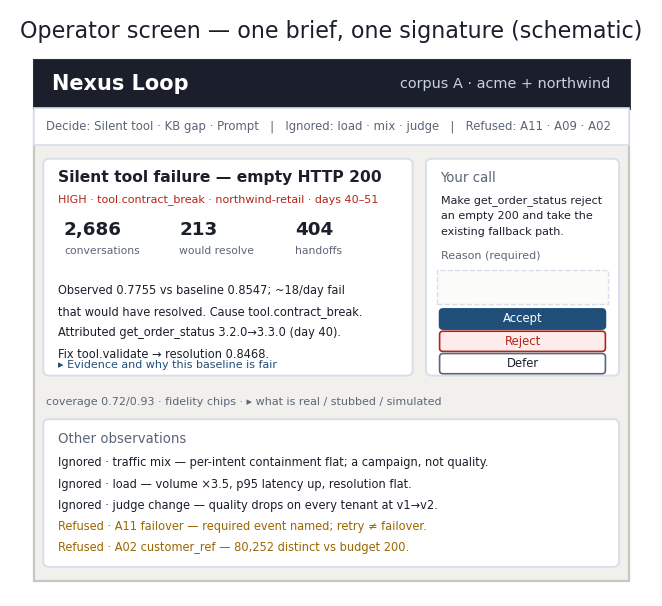
\includegraphics[width=0.98\columnwidth]
    {figures/operator_screen.png}
    \caption{
        Final operator-facing screen showing the finding, evidence,
        proposed fix, and approval/rejection control.
    }
    \label{fig:screen}
\end{figure}

The screen communicates:

\begin{itemize}
    \item What went wrong;
    \item Who was affected;
    \item Evidence supporting the finding;
    \item Baseline and computation;
    \item Diagnosis;
    \item Proposed fix;
    \item Risk;
    \item Verification result;
    \item Approve / Reject decision.
\end{itemize}

Explain how a new operator could determine the appropriate action
without requiring assistance from the development team.

% =========================================================
% 17. FAILURE CASES AND LIMITATIONS
% =========================================================

\section{Failure Cases and Limitations}

\subsection{Known Failure Cases}

Discuss cases where the system:

\begin{itemize}
    \item Missed a genuine regression;
    \item Produced an uncertain diagnosis;
    \item Could not establish a valid baseline;
    \item Could not measure an important metric;
    \item Proposed an ineffective fix;
    \item Required human intervention.
\end{itemize}

\subsection{Scale Limitations}

Describe what breaks or becomes expensive at approximately
\textbf{100$\times$ the current scale}.

Consider:

\begin{itemize}
    \item Data volume;
    \item Storage;
    \item Query complexity;
    \item Model inference cost;
    \item Replay cost;
    \item Search space;
    \item Human review burden.
\end{itemize}

Clearly distinguish between components that are implemented and those
that are simulated or stubbed.

% =========================================================
% 18. ASSUMPTIONS AND TRANSPARENCY
% =========================================================

\section{Assumptions and Transparency}

Explicitly state:

\begin{itemize}
    \item What is fully implemented;
    \item What is stubbed;
    \item What is simulated;
    \item What uses a language model;
    \item What is directly measured from logs;
    \item What is derived from measured quantities;
    \item What is judged by a model;
    \item What requires human input;
    \item What does not work at larger scale.
\end{itemize}

No metric definition, judge version, or reviewed ``good'' set is changed
to improve the reported result.

% =========================================================
% 19. REPRODUCIBILITY
% =========================================================

\section{Reproducibility}

\subsection{Execution Procedure}

Provide the minimum steps required to reproduce the sealed-run output.

\begin{enumerate}
    \item [Step 1: Environment setup]
    \item [Step 2: Dataset / configuration]
    \item [Step 3: System execution]
    \item [Step 4: Report generation]
    \item [Step 5: Schema validation]
    \item [Step 6: Screen launch]
\end{enumerate}

\subsection{Generated Artifacts}

The submission contains:

\begin{itemize}
    \item \texttt{loop-report.json};
    \item Complete system source code;
    \item Operator-facing screen;
    \item README / execution instructions;
    \item [Additional files].
\end{itemize}

The final report must be generated by the system without manual edits.

% =========================================================
% 20. CONCLUSION
% =========================================================

\section*{Conclusion}

We presented \textbf{[SYSTEM NAME]}, an autonomous improvement loop for
AI-agent deployments. The system connects detection, diagnosis,
prescription, verification, and human decision-making into a single
workflow.

The final system identifies \textbf{[X]} genuine problems, correctly
dismisses \textbf{[X]} lookalikes, reports \textbf{[X]} measurement
gaps, and verifies \textbf{[X]} proposed fixes. It achieves
\textbf{[KEY RESULT]} while maintaining \textbf{[RUNTIME]} runtime and
\textbf{[COVERAGE]} coverage.

The central contribution is not merely anomaly detection, but a
traceable improvement loop in which every important number has a
defined provenance, every diagnosis is supported by evidence, proposed
changes are verified, and the final action remains in human hands.

% =========================================================
% REFERENCES
% =========================================================

\begin{thebibliography}{9}

\bibitem{YellowAI}
Yellow.ai,
\textit{Nexus Loop -- TECHQUEST Problem Statement Series},
Product Development \& Agentic AI.

\bibitem{Kit}
Yellow.ai,
\textit{Nexus Loop Kit, Schema, Examples and Replay Service},
Provided Challenge Resources.

\bibitem{Method1}
[Author(s)],
\textit{[Primary Method / Algorithm Used]},
[Year].

\bibitem{Method2}
[Author(s)],
\textit{[Root Cause Analysis / Agent Evaluation Method]},
[Year].

\bibitem{Method3}
[Author(s)],
\textit{[Model / Judge / Retrieval Method Used]},
[Year].

\end{thebibliography}

\end{document}
